\documentclass{../weeklyslides}

\addbibresource{../../References.bib}

\title[Weekly Report]{ECE 497: Special Project \\ Weekly Report}
\subtitle{Week 04}
\author{Alexander Lukens \and Karl Hallsby}
\institute{Illinois Institute of Technology}
\date{\DTMdisplaydate{2021}{2}{18}{-1}}

\begin{document}

\nocite{chipyard}

\begin{frame}
  \titlepage{}
\end{frame}

\section{What We Did}\label{sec:What_We_Did}
\begin{frame}
  \frametitle{\nameref*{sec:What_We_Did}}
  \begin{itemize}
  \item Attempted to flash default chip to Alex's FPGA.\@
  \item Successfully passed USB connection to FPGA through to VirtualBox VM, interfaced with FPGA in Vivado
  \item Conducted ``Hello World'' project on FPGA to ensure that bitstream was being sent to FPGA correctly.
  \item Used FPGA Prototyping Flow in Chipyard to generate a bitstream for the Arty FPGA board.
    Strangely, the default ``example'' project for the Arty did not pass all timing constraints.
    \begin{itemize}
    \item Will require additional investigation
    \end{itemize}
  \item When creating bitstream in Chipyard, Vivado runs several tests on the design and produces detailed reports in a Chipyard folder.
  \end{itemize}
\end{frame}

\section{What We Learned}\label{sec:What_We_Learned}
\begin{frame}
  \frametitle{\nameref*{sec:What_We_Learned}}
  \begin{itemize}
  \item The repository is incredibly complicated
  \item \textbf{VERY} deep directory nesting (Partly due to Scala/Java project directory conventions).
  \item Putting the generated chip on an FPGA seems to be much more difficult than originally thought.
  \item Generating a non-default chip can be very easy or very hard.
    \begin{itemize}
    \item Some of the options that must be overridden to ensure a different chip is built and simulated/benchmarked are not easy to understand or find.
    \end{itemize}
  \end{itemize}
\end{frame}
\begin{frame}
	\frametitle{\nameref{sec:What_We_Learned}}
	\begin{itemize}
	\item Generating Custom SoC configurations requires lots of memory. Will likely upgrade my computer to meet requirements (16GB $\rightarrow$ 32+ GB)
	\item Successfully created custom config file using building blocks provided by Chipyard, produced 8-core "small Rocket core" SoC with otherwise default settings
	\item Utilized RISC-V toolchain to compile basic test program (hello world plus simple for loop)
	\end{itemize}
\end{frame}

\begin{frame}
	
\begin{figure}
	\centering
	\includegraphics[width=0.9\linewidth]{"Baremetal RISCV instr"}
	\caption{Commands to compile for RISC-V Simulator}
	\label{fig:baremetal-riscv-instr}
\end{figure}

\end{frame}

\begin{frame}
	
\begin{figure}
	\centering
	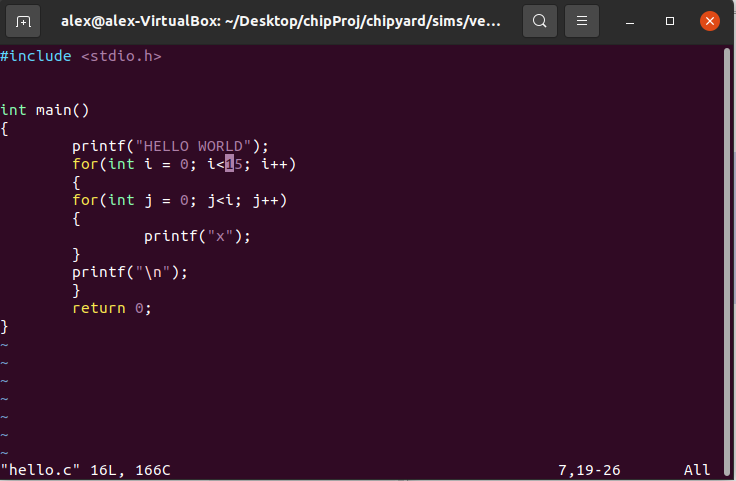
\includegraphics[width=0.5\linewidth]{helloC}
	\caption{hello.c code}
	\label{fig:helloc}
\end{figure}

\begin{figure}
	\centering
	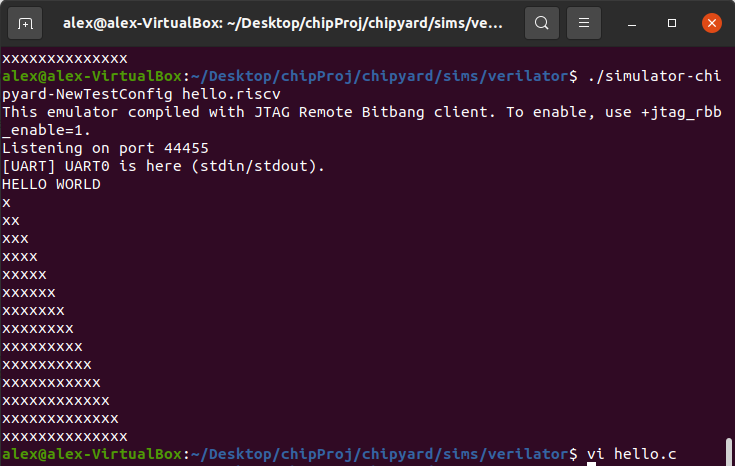
\includegraphics[width=0.5\linewidth]{helloCout}
	\caption{hello.c output from simulator}
	\label{fig:hellocout}
\end{figure}

	
\end{frame}




\section{Next Steps}\label{sec:Next_Steps}
\begin{frame}
  \frametitle{\nameref*{sec:Next_Steps}}
  \begin{itemize}
  \item Continue trying to write the default chip out to Alex's FPGA and test.
  \item Using Alex's discovery in Vivado, collect gate counts of components within the default chip.
  \item Practice generating other non-default chips to understand all the options used when generating a new chip.
  \item Hopefully, start defining a new, custom, chip using what we know, and building a \emph{very} small proof-of-concept.
  \end{itemize}
\end{frame}

\begin{frame}
  \frametitle{References}
  \printbibliography[heading=bibintoc]{}
\end{frame}

\end{document}

%%% Local Variables:
%%% mode: latex
%%% TeX-master: t
%%% End:
